\subsection{Modelo}

Recall that the main objective of accessing the data is to obtain knowledge, to understand and make sense of it. Of course, 
pure data by itself has no value until we can understand it and apply it. We must contextualize, process, and analyze the 
information to gain useful knowledge. \\
    
\begin{figure}[ht]
    \centering 
    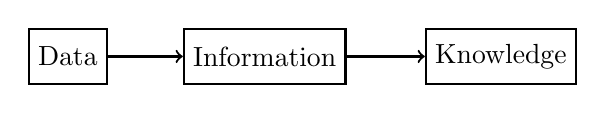
\begin{tikzpicture}[thick]
        \node[draw,rectangle,minimum size=20] (a) {Data};
         \node[draw,rectangle,minimum size=20,right of= a, node distance=2.5cm] (b) {Information};
         \node[draw,rectangle,minimum size=20,right of=b, node distance=3cm] (c) {Knowledge};
         \draw[->] (a) to (b);
        \draw[->] (b) to (c);
     
      \end{tikzpicture}
      \caption{Diagrama. De datos a conocimiento}
    \end{figure}
 
    In order to obtain this knowledge, the user must correctly interpret the data. It's not enough to know what the values and 
    units individually represent, but what they mean in the big picture. For that the user must already have expertise in the 
    area, or must engage in further research allowing them to understand the data that has been extracted.
     
    In order to build a system that makes data accessible, it is essential to design a model to specify the
    information that we want to obtain. The design of a system will allow that, based on given values, provide some results.
    For this it will be necessary to have a solid knowledge of the dataset that is needed, the values,
    their units and how they relate to each other.


\subsubsection{How to solve it} 
Study the objective sought and resort to the help of experts if necessary to acquire the necessary knowledge
on the subject. Design a model that provides the information we are looking for.

\subsubsection{How we solve it. Aire Guru} 
Aire Guru aims to increase the awareness of the level of pollution that surrounds us. To do this, it uses a measure called
the air quality index (AQI), specifically the European air quality index (EAQI).


\newpage
\begin{figure}[ht]
    \centering
    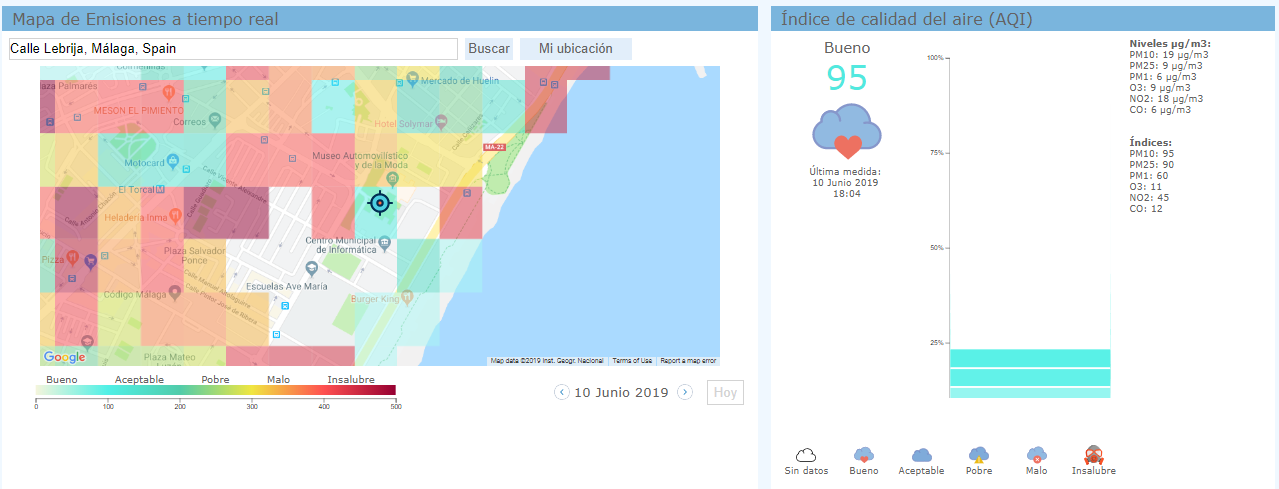
\includegraphics[width=10cm]{mapAireGuru}
    \caption{Aire Guru. Landing page. Top section}
\end{figure}

It shows the AQI in the whole city of Málaga by zones, both the general and the AQI of each of the 
pollutans in a more disaggregated form from September 2018 to the present. It also shows the evolution
of these for days, months and years.
It is capable of creating a set of the most relevant pollutans by medical condition. An innovative feature is the capacity to display levels of any particular pollutant by hour, day, month, or year. 

\elsparagraph{Evaluation}  

\begin{itemize}
\done The information is focused on an objective, informing the user of the level of pollution that surrounds them, both  in real time
and in the past.
\done The information follows a logical thread; it tells a story.
\done The web offers understandabl, useable information, not just raw data.
\end{itemize}

\newpage